\documentclass[a4paper, 11pt]{article}
\usepackage{amsmath}
\usepackage{amsfonts}
\usepackage{amssymb}
\usepackage{caratula}
\usepackage[spanish, activeacute]{babel}
\usepackage[usenames,dvipsnames]{color}
\usepackage[width=15.5cm, left=3cm, top=2.5cm, height= 24.5cm]{geometry}
\usepackage{graphicx}
\usepackage[utf8]{inputenc}
\usepackage{listings}
\usepackage[all]{xy}
\usepackage{multicol}
\usepackage{subfig}

\usepackage{cancel}
\usepackage{float}
\usepackage{xcolor}
\usepackage{color,hyperref}

\usepackage{multirow} % para las tablas


%%%%%%%%%%%%%% ALGUNAS MACROS %%%%%%%%%%%%%%
% For \url{SOME_URL}, links SOME_URL to the url SOME_URL
\providecommand*\url[1]{\href{#1}{#1}}

% Same as above, but pretty-prints SOME_URL in teletype fixed-width font
\renewcommand*\url[1]{\href{#1}{\texttt{#1}}}

% Comando para poner el simbolo de Reales
\newcommand{\real}{\hbox{\bf R}}

\providecommand*\code[1]{\texttt{#1}}

%uso: \ponerGrafico{file}{caption}{scale}{label}
\newcommand{\ponerGrafico}[4]
{\begin{figure}[H]
	\centering
	\subfloat{\includegraphics[scale=#3]{#1}}
	\caption{#2} \label{fig:#4}
\end{figure}
}

%\renewcommand{\algorithmiccomment}[1]{\hfill #1}

%%%%%%%%%%%%%%%%%%%%%%%%%%%%%%%%%%%%%%%%%%%%

\materia{Ingeniería de Software II}

\titulo{Big Tiza}
%\fecha{fecha de entrega}
%\grupo{Nro grupo}
\integrante{Agustina Ciraco}{630/06}{agusciraco@gmail.com}
\integrante{Alejandro Rebecchi}{15/10}{alejandrorebecchi@gmail.com}
\integrante{Maria Lara Gauder}{27/10}{marialaraa@gmail.com}
\integrante{Martin Heredia}{146/11}{martin.herediaf@gmail.com}

\include{templates}

\begin{document}
\pagestyle{myheadings}
\maketitle
%\markboth{Nombre materia}{Nombre TP}

\thispagestyle{empty}
\tableofcontents

%\setcounter{section}{-1}
\newpage

\section{Introducci\'on}

En este trabajo práctico se presentan Las arquitecturas del sistema correspondiente a la primera entrega (versión para escuela de villa urquiza) y la correspondiente al sistema pedido por el ministro, cuyo alcance es a nivel pais.
Se detallan Los atributos de calidad pedidos, junto con sus respectivos escenarios. Por otro lado se presenta una discusión sobre las diferencias entre las metodologías utilizadas en cada tp, y por último conclusiones.
\newpage
\section{Atributos de Calidad}
\subsection{Listado atributos de calidad pedidos}
\begin{itemize}
\item[Performance] Monitorear el estado de las campañas de manera agil. No se admiten demoras de ningún tipo .
\item[Disponibilidad] Fallas de comunicación durante transición de servidores
\item[Modificabilidad] Cambio de servidores entre etapa de Cordoba a etapa pais.
\item[Seguridad]Proteger datos y modificación (campañas y evaluación).
\item[Seguridad]Auditar
\item[Disponibilidad] Envio de mensajes. (Patagonia)
\item[Certeza de Datos] Para la estimacion de campanias
\item[Modificabilidad-Scalabilidad] Volumen de datos
\item[Performance-Scalabilidad] Mantener el 80 porciento de tiempo de envio.
\item[Modificabilidad] Campanias privadas
\item[Flexibilidad] politica nacional de metricas
\item[Usabilidad] Crear campanias
\item[Usabilidad] Visualizar campanias
\item[Usabilidad] Visualizar Resultados
\end{itemize}
\subsection{Escenarios de Atributos de calidad}
\begin{table}[H]
\centering
\begin{tabular}{ | p{5cm} | p{8cm} | p{1.5cm} | }
\hline
Clasificación & Caso de Uso & Horas H.\\ \hline \hline
\multirow{2}{5cm}{Usuarios} & Ingresando al sistema & 36 \\ \cline{2-3}
& Cargando usuario & 13 \\ \hline
%~ & Importando suscripciones& 13 \\ \hline
Eventos & Creando Evento & 7 \\ \hline
\multirow{2}{5cm}{Campañas} & Creando Campaña & 29 \\ \cline{2-3}
& Evaluando Campañas & 18 \\ \hline
\multirow{3}{5cm}{Administración de mensajes} & Enviando Mensajes & 32 \\ \cline{2-3}
& Recibiendo respuesta & 25 \\ \cline{2-3}
& Programando envio de mensajes & 16 \\ \hline
\multirow{4}{5cm}{Destinatarios} & Creando Destinatario & 14 \\  \cline{2-3}
& Modificando datos de Destinatario & 11 \\ \cline{2-3}
& Cancelando Suscripci\'on & 10 \\ \cline{2-3}
& Suscribiendo destinatario a una campaña & 10 \\ \hline
\multirow{3}{5cm}{Resultados} & Cargando Resultado de Campaña & 11 \\ \cline{2-3}
& Comparando Campañas & 14 \\ \cline{2-3}
& Eligiendo métrica & 5 \\ \hline
\multirow{4}{5cm}{Visualización} & Visualizando Campaña & 20 \\ \cline{2-3}
& Visualizando Evento & 20 \\ \cline{2-3}
& Visualizando Resultados & 20 \\ \cline{2-3}
& Visualizando Destinatario & 20 \\ \hline

\end{tabular}
\end{table}


\newpage

\section{Arquitecturas}
\subsection{Arquitectura TP1}
A partir del proyecto Aula al 2020, de los objetivos planteados y el prototipo desarrollado, se define el siguiente diagrama de arquitectura:

\centerline{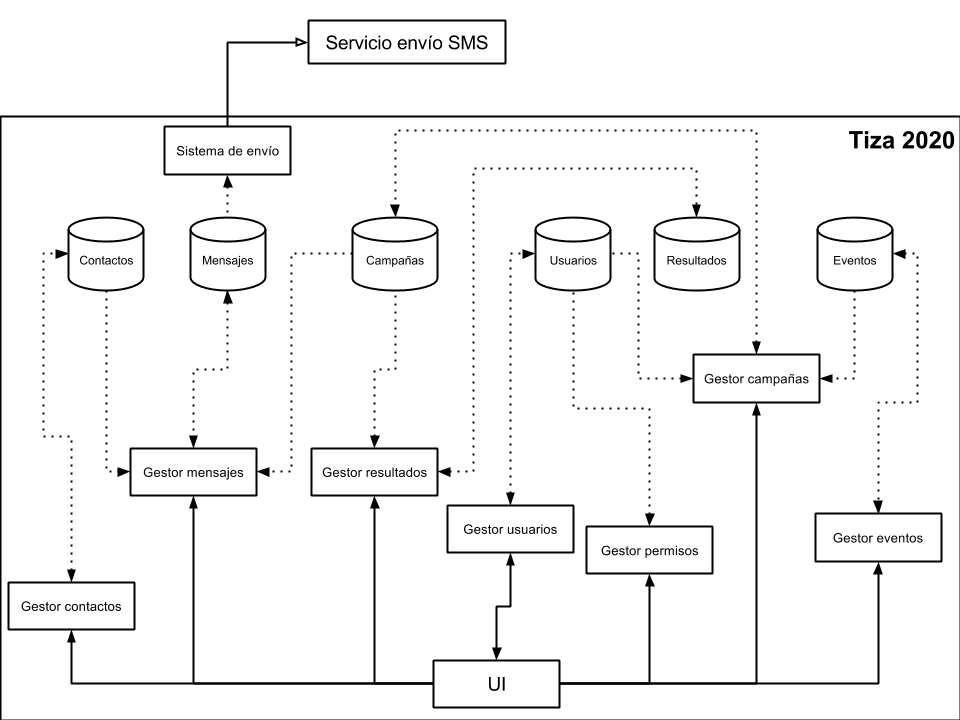
\includegraphics[width=1.2\textwidth]{./diagramas/ArquitecturaTP1.png}}
\centerline{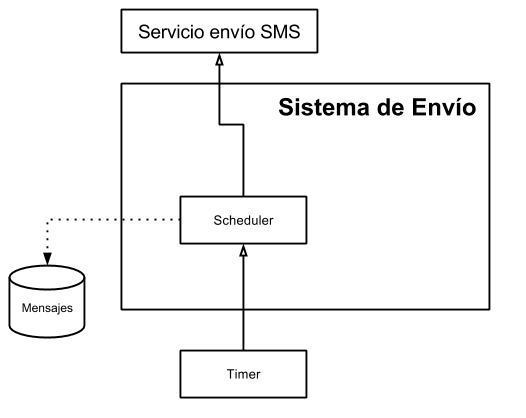
\includegraphics[width=0.5\textwidth]{./diagramas/ArqTP1SistEnvio.png}}

En primer lugar se presenta la UI, que es la encargada de la interacción del usario con el sistema de Tiza 2020. La misma recibe los pedidos por parte del usuario. Para comenzar, se deberá validar el acceso del mismo, es decir, verificar su previa inscripción en el sistema. Para eso el UI indica al ''Gestor usuarios'' el id del usuario que intenta acceder. Este último lee la base de datos, buscando los datos del mismo. En caso de no existir, retorna al UI un aviso de usuario inválido, el cual se encargará de notificarle a la persona. Caso contrario, responde que se permite el acceso al usuario al sistema. 
En caso de que el usuario sea válido, el UI envía un pedido al "Gestor campañas", pidiendo las campañas correspondientes al usuario para poder mostrarlas como el siguiente menú, luego del inicio de sesión. El componente "Gestor campañas", pide del repositorio las campañas que tienen en el campo de "usuario con permiso de acceso" al id del usuario. Luego, envía la información de todas las campañas, completándolo con los datos requeridos en los demás repositorios, como podría ser el caso de los teléfonos de los contactos. 
El proceso se repite para cada menú que el usuario desee ver. Además, el gestor se encargará de recolectar la información necesaria y traducirla a una interfaz para que sea comprensible por el usuario y se le enviará al UI, quien se encarga de mostarla. En el caso de de que se desee mostrar la agenda correspondiente a un usuario, para poder incluirlo en la creación de un mensaje, el UI pedirá al "Gestor contactos", la información necesaria. Este último se encargará de acceder a la base de datos y recolecctar los datos pedidos. El proceso es el mismo para el "Gestor mensajes", "Gestor resultados", "Gestor eventos", siendo cada uno el encargado de interpretar para el UI los datos necesarios y de armar la interfaz necesaria. 

Por otro lado, cuando un usuario, tanto Docente como personal de la Secretaría o Dirección, desean crear o modificar algún objeto del sistema, lo indicarán al UI, utilizando los accesos que correspondan, y este se encargará de avisar al gestor que corresponda con el objeto. El gestor correspondiente se encargará de agregar el nuevo objeto al repositorio necesario.  En caso de que se desee modificar uno existente, también levantará de la base de datos el objeto, le aplicará la modificación indicada por el usuario y lo volverá a cargar en el repositorio. 

El "Sistema de envío" es el encargado de enviar los mensajes. El "Timer" le envía cada hora un mensaje asincrónico al "Scheduler" con la hora y fecha actuales. El "Scheduler" se encargará de leer en la base de datos aquellos menajes que cumplan con esa hora y fecha de envío. Al obtener todos los mensajes, los traducirá para poder ser interpretados por el "Servicio envío SMS". Este último es un sistema externo que se contratará para cumplir la función de enviar los SMS necesarios. 
\subsection{Arquitectura TP2}
La arquitectura de esta parte se realizó contemplando los atributos de calidad nombrados en la sección anterior. A continuación se muestra el diseño realizado para esta parte, seguido de un detalle de desiciones tomadas.

\emph{Desición de Diseño} Al momento de contemplar el atributo de calidad de \textbf{Disponibilidad} respecto el envío de mensajes, se tomó la decisión de realizar la conexión entre componete servicio mensajeria  y el componente, de lado de Big tiza, de envio de mensajes, mediante 2 conectores distintos. Dado que se tiene en cuenta que al momento  de enviar mensajes, puede fallar la conexión con los distintos servicios (twitter facebook, sms). 
Se optó por crear 2 conectores para esta unión, uno que muestra la conxión normal, sin fallas y otro la conexión considerando falla de comunicación. 
Viendo en detalle el conector del camino sin fallas se puede observar que existe un traductor para poder comunicarse con cada tipo de servicio (facebook, twiter etc) ya que cada uno tiene un formato distinto.
En el caso del conector de camino alternativo (2), que contempla la falta de conexion, al ver el conector más en detalle se puede observar  que se tiene el componente servicio alternativo de mensajería, quién se encarga de tomar la decición correspondiente y conectarse con el servicio de la empresa de telefonia privada para poder concretar el envío.

%revisar que decision tomamos respecto a la version de oca
Además en este caso se contempló un tercer caso que coincide con el análisis de riesgo, tomado para la parte de planificación, donde se considera una conexión directa con un servicio de correo (oca), para poder contar con él en el caso de no tener ningún tipo de conexión con los otros servicios. %de esa manera se desliga el sistema Big tiza de esa responsabilidad.

Al considerar las situaciones de envío de camino sin fallas, donde como hay que evitar el uso de la empresa de telefonía privada, ya que esta puede generarle costos a los receptores, lo cual se desea evitar, por lo que se van a hacer varios intentos, antes de tomar la desición de cambiar de conector.

%~ Para la decision de por donde enviar se la asigna a un componente dentro de componente de envio de mensajes, esto se pude observar al hacer zoom de este comp 

\emph{Desicisión de Diseño}
Al momento de contemplar en las respuestas de aquellas campañas que esperar respuestas a los mensajes enviados, se asume que los mensajes se envían con un código para vincular con dicha campaña, para de esta manera poder generar los resultados correspondientes.

Por otro lado, se optó por tener un componente \textbf{Servicio de evaluacion de estadisticas}, el cual es externo con el cual hay que conectarse al momento de evaluar los resultados, el mismo es definido por cada municipio acorde a lo que se desee evaluar (campaña de saludo, de educacion vial, etc)

Otra parte importante a la hora de hablar de la arquitectura de Big Tiza, es la parte del procesado de resultados de las campañas, ya que esta parte involucra 2 partes importantes, la de procesado de campañas y la parte de visualizarlos en por ejémplo un dashboard.
En cuando al procesado de los resultados, primero hay que considerar cómo llegan al sistema, una opción posible es la carga manual de dichos resultado. Esta opción es considerada dado que el 
Los resultados de las campañas pueden ser cargados manualmente a travez del componente gestor de resultados(considerando aquellas campanias que no reciben respuesta para evaluar) para poder ser evaluados.



%~ Los resultados son los efectos de la campania, por ejemplo el apropbo pepe el examen, ese resultado es evaluado y dice aprobo la mitad, y eso es contrastado con una metrica lo cual define la conclusion de una campania, por ejemplo aprobo el 80 porciento y ese porcentaje es bueno o malo respecto a la metrica que se definio, y eso se muestra en esta visualizacion constante de las campanias
%~ 
%~ Las evaluaciones se guardan para futuras consultas, aunque se haya finalizado la campania.
%~ 
%~ Al agregar el web browser asumimos que en ese camino se contemplan los permisos de usuario, y al este solo interactuar con el web server no hay que contemplar otro caso de seguridad en este aspecto de permisos.
%~ 
%~ 
%~ En el caso de los componentes que no se acceden a travez del usuario (web server), se contempla que esten preparados para evitar el robo de datos. Por ejemplo, el componente de recepcion de mensajes de resultado de campanas, ya que reciben mensajes por fuera, y alguno podria ser un potencial ataque de seguridad. pero para evitar esto se considera que se realiza un chequeo de seguridad previo a ingresarlo a la base de datos.
%~ 
%~ 
%~ 
%~ Gestor del dashboard Este componente tiene 2 caminos la muestra del tiempo real y la muestra de los resultados finalizados
%~ 
%~ Esto va mas que nada a que todo el tiempo se tiene que estar mostrando el resultado de la campania y dado que aca estamos considerando big data no se puede tener en tiempo razonable el resultado final. Por ello se van mostrando resultados parciales que se van extrapolando a un resultado porcentual respecto de la poblacion, (ya que es un resultado puntual pero se quiere mostrar a nivel poblacion)
%~ Entonces el camino de procesamiento.
%~ Esto sirve para los escenarios de performance
%~ 
%~ En cuanto a disponibilidad se habla de los conectores distinto
%~ 
%~ 
%~ gestor de campanias ahi comentar el atributo de modificabilidad respecto de campanias privadas


\subsection{Discusión de Arquitecturas}

\newpage
\section{Discusión Metodologías}
\subsection{Metodologías TP1}
\subsection{Metodologías TP2}
\subsection{Diferencias}

\newpage
\section{Conclusiones}

\end{document}
